\documentclass{article}
\usepackage{graphicx}
\usepackage[a4paper, margin=3cm]{geometry}
\usepackage{fancyhdr}
\usepackage{lastpage}
\usepackage{hyperref}
\usepackage{polski}
\usepackage{amsmath}
\usepackage{blindtext}
\usepackage{multicol}
\usepackage{listings}

\title{Wprowadzenie do cyberbezpieczeństwa\\Temat 1:\\Uwierzytelnianie klienta SSH\\za pomocą kluczy prywatnych}
\author{Jakub Stachowicz, 198302\\Jan Wiśniewski, 197662}
\date{26 maja 2025}

\pagestyle{fancy}
\fancyhf{} % Clear header and footer
\fancyfoot[C]{Strona \thepage\ z \pageref{LastPage}}

\renewcommand{\headrulewidth}{0pt} % Remove the horizontal bar at the top
\renewcommand{\footrulewidth}{0pt} % Remove the horizontal bar at the bottom if needed

\renewcommand{\contentsname}{Spis rzeczy} % Change the TOC title

\newcounter{firstbib} % New couter for bibliografy

\begin{document}
\maketitle
\newpage
\tableofcontents
\newpage


\begin{multicols}{2}
[
\section{Omówienie SSH i konfiguracja serwera}
]
\subsection{Czym jest SSH?}
SSH (Secure Shell) to protokół sieciowy, który służy do zdalnego logowania się do innego komputera (serwera) w sposób bezpieczny. Umożliwia zarządzanie systemem operacyjnym, przesyłanie plików oraz wykonywanie poleceń na odległość -- wszystko to przy użyciu szyfrowanego połączenia\cite[The SSH protocol]{whatisssh}.

Uwierzytelnianie w SSH może odbywać się na dwa sposoby: za pomocą hasła lub kluczy kryptograficznych. Logowanie hasłem jest proste, ale mniej bezpieczne, ponieważ narażone jest na ataki typu brute-force. Znacznie bezpieczniejszą i częściej stosowaną metodą jest logowanie przy użyciu kluczy SSH, które opiera się na parze klucz prywatny–publiczny. Klucz publiczny umieszczany jest na serwerze, a prywatny pozostaje na komputerze użytkownika, dzięki czemu możliwe jest uwierzytelnienie bez podawania hasła. Metoda ta jest szczególnie przydatna w automatyzacji i pracy z wieloma serwerami\cite[Automate with SSH keys, but manage them]{whatisssh}.

\subsection{Algorytmy kryptograficzne w SSH}
Temat algorytmów kryptograficznych w protokole SSH dotyczy zarówno szyfrowania samego ruchu sieciowego między klientem a serwerem, jak i logowania i autoryzacji. Niniejsze opracowanie skupia się na algorytmach stosowanych w autoryzacji za pomocą kluczy prywatnych.

W protokole SSH można używać kilku algorytmów generujących parę kluczy, w standardzie zdefiniowano RSA, DSS (DSA) oraz umożliwiono definiowanie innych kluczy\cite[6.6.~s.~13]{rfc4253}. Najpopularniejsze to RSA, ECDSA i Ed25519 (a dawniej używano też DSA, które dziś jest uważane za przestarzałe). OpenSSH wspiera następujące typy kluczy: DSA, RSA, ECDSA oraz Ed25519\cite[User key generation]{learnms}. Obecnie zaleca się wybór silniejszych algorytmów, np. RSA lub Ed25519 -- OpenSSH 7.0 i nowsze domyślnie wyłączają słaby DSA, a od wersji 10.0 wsparcie dla tego algorytmu zostało usunięte w całości\cite{openssh10}.

Dalsza część artukułu skupia się na użyciu kluczy RSA, jednak pozostałych algorytmów można użyć w bardzo podobny sposób. Najczęściej -- poprzez zmianę parametru \verb|rsa| na np. \verb|ed25519|.

\subsection{Konfiguracja z wymuszonym użyciem kluczy}
Aby serwer SSH (usługa \verb|sshd|) zezwalał tylko na logowanie kluczem i wyłączał logowanie hasłem, należy zmodyfikować plik konfiguracyjny znajdujący się najczęściej pod ścieżką \verb|/etc/ssh/sshd_config|\cite{sshconfig}. Ważne dyrektywy to m.in.:
\begin{enumerate}
    \item \verb|PubkeyAuthentication yes| -- włącza uwierzytelnianie kluczem publicznym (domyślnie zazwyczaj jest włączone).
    
    \item \verb|PasswordAuthentication no| -- wyłącza logowanie hasłem. Po jego ustawieniu serwer nie akceptuje haseł SSH.

    \item \verb|AuthorizedKeysFile| -- określa lokalizację pliku z kluczami publicznymi (domyślnie dla parametru \verb|%h/.ssh/authorized_keys| będzie to \verb|~/.ssh/authorized_keys|).
\end{enumerate}

\noindent
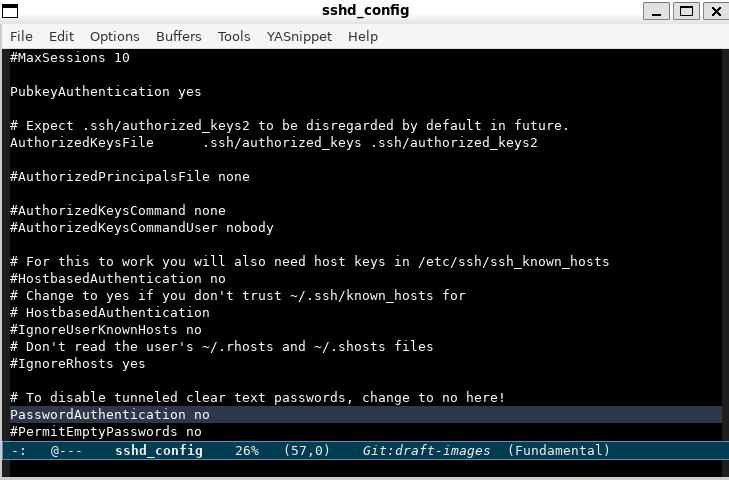
\includegraphics[width=\linewidth]{sshd_config.png}

Po edycji pliku \verb|sshd_config| należy zapisać zmiany i ponownie uruchomić serwis SSH, np.: \verb|sudo systemctl restart sshd| lub \verb|sudo service sshd reload|. Spowoduje to zastosowanie nowych ustawień. 

\noindent
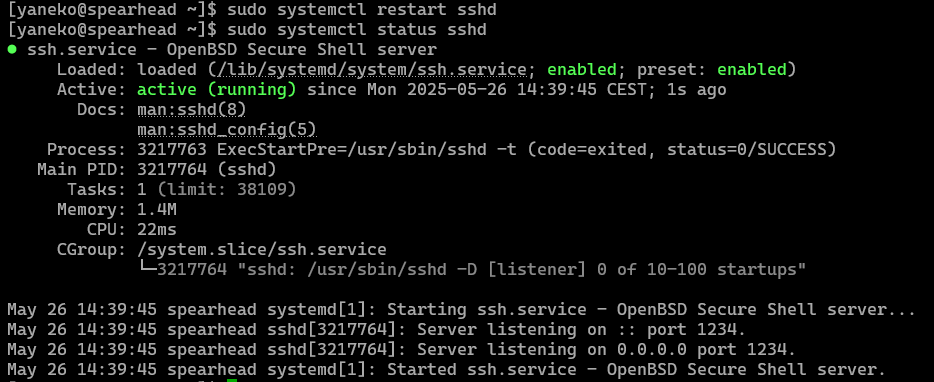
\includegraphics[width=\linewidth]{system_d.png}

\end{multicols}

\newpage
\begin{multicols}{2}
[
\section{Klucze -- generowanie i instalacja}
]
\subsection{Generowanie kluczy}
Parę kluczy (klucz prywatny i publiczny) generuje użytkownik. Klucz prywatny przechowywany jest po stronie klienta, natomiast klucz publiczny -- po stronie serwera.

\subsubsection{W systemie Linux -- ssh-keygen}
W Linuksie (oraz systemach UNIX/macOS) zwykle używa się polecenia \verb|ssh-keygen|. Przykładowo:
\verb|ssh-keygen -t rsa -b 4096|. Polecenie \verb|-t rsa -b 4096| tworzy klucz RSA o długości 4096 bitów\cite{sshkeygen}. 

Po uruchomieniu program zapyta o ścieżkę do pliku (domyślnie \verb|~/.ssh/id_rsa| dla RSA lub \verb|~/.ssh/id_ed25519| dla Ed25519) i opcjonalne hasło (passphrase). Gdy zakończy generowanie, w katalogu \verb|~/.ssh/| powstaną dwa pliki: \verb|id_rsa| (klucz prywatny) i \verb|id_rsa.pub| (klucz publiczny).

\noindent
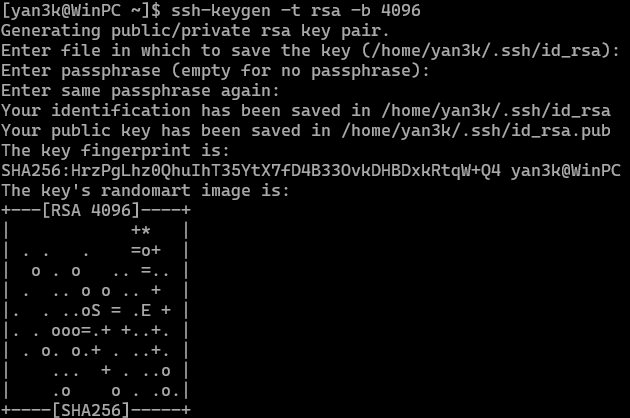
\includegraphics[width=\linewidth]{ssh_keygen_rsa_4096.png}

\subsubsection{W systemie Windows -- PuTTYgen}
W systemie Windows często korzysta się z PuTTYgen (narzędzie wchodzące w skład pakietu PuTTY). Uruchamiamy PuTTYgen, wybieramy typ klucza (np. RSA lub Ed25519) i długość (np. 2048 bitów), a następnie klikamy przycisk Generate. PuTTYgen poprosi nas o losowe ruchy myszką w obrębie okna -- to sposób na zebranie entropii do generacji klucza. Gdy pasek postępu dojdzie do końca, w oknie PuTTYgen pojawi się wygenerowany klucz publiczny (tekst zaczynający się np. \verb|ssh-rsa AAAA...|). 

\noindent
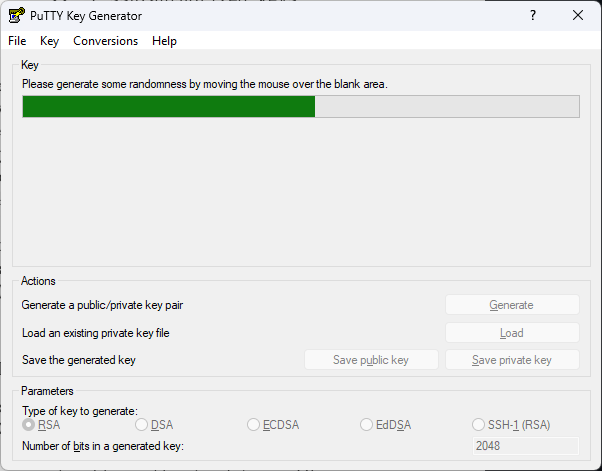
\includegraphics[width=\linewidth]{putty_gen.png}

Następnie należy wpisać (dwukrotnie) passphrase chroniący klucz prywatny (zalecane) i zapisać pliki: kliknąć Save public key (np. \verb|mykey.pub|) oraz Save private key (plik \verb|.ppk| dla PuTTY, np. \verb|mykey.ppk|).

\noindent
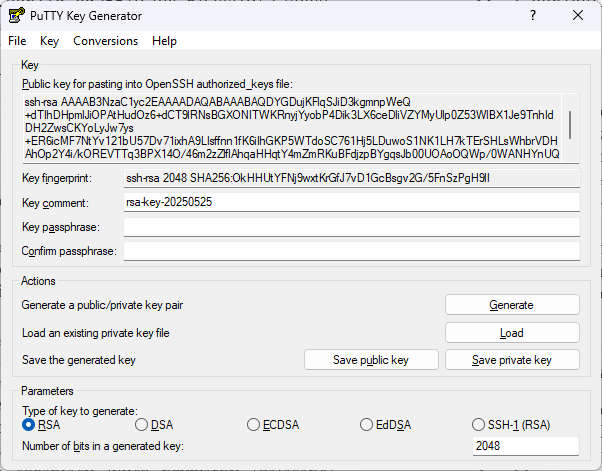
\includegraphics[width=\linewidth]{putty_gen-finished.png}

W PuTTYgenie można też przekonwertować prywatny klucz do formatu OpenSSH (menu Conversions →
Export OpenSSH key) -- przydaje się to, gdy chcemy używać tego samego klucza w programach innych niż
PuTTY. Plik \verb|.ppk| pozostaje natywnym formatem PuTTY. 

\noindent
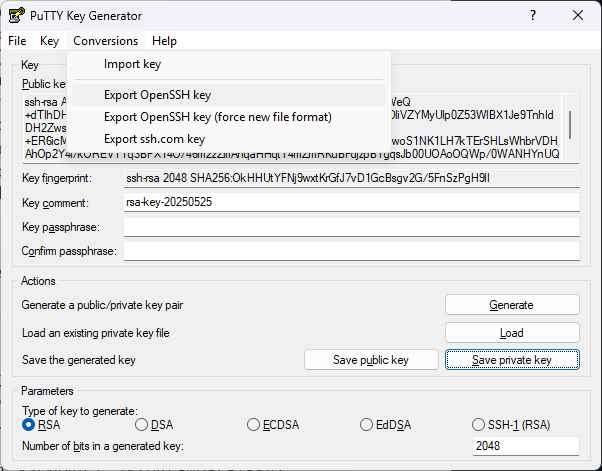
\includegraphics[width=\linewidth]{putty_gen-export_openssh.png}

\subsection{Instalacja kluczy}
Po wygenerowaniu kluczy należy je zainstalować -- zarówno po stronie klienta, jak i serwera.

\subsubsection{Klient i serwer SSH Linux}
Aby klient logujący się z Linuksa mógł użyć swojego klucza, klucz publiczny klienta należy dodać do pliku
\verb|~/.ssh/authorized_keys| konta docelowego na serwerze. Najprościej to zrobić poleceniem \verb|sshcopy-id| -- narzędzie automatycznie kopiuje nasz klucz publiczny do odpowiedniego pliku na serwerze. Przykład: \verb|ssh-copy-id user@serwer|.

\noindent
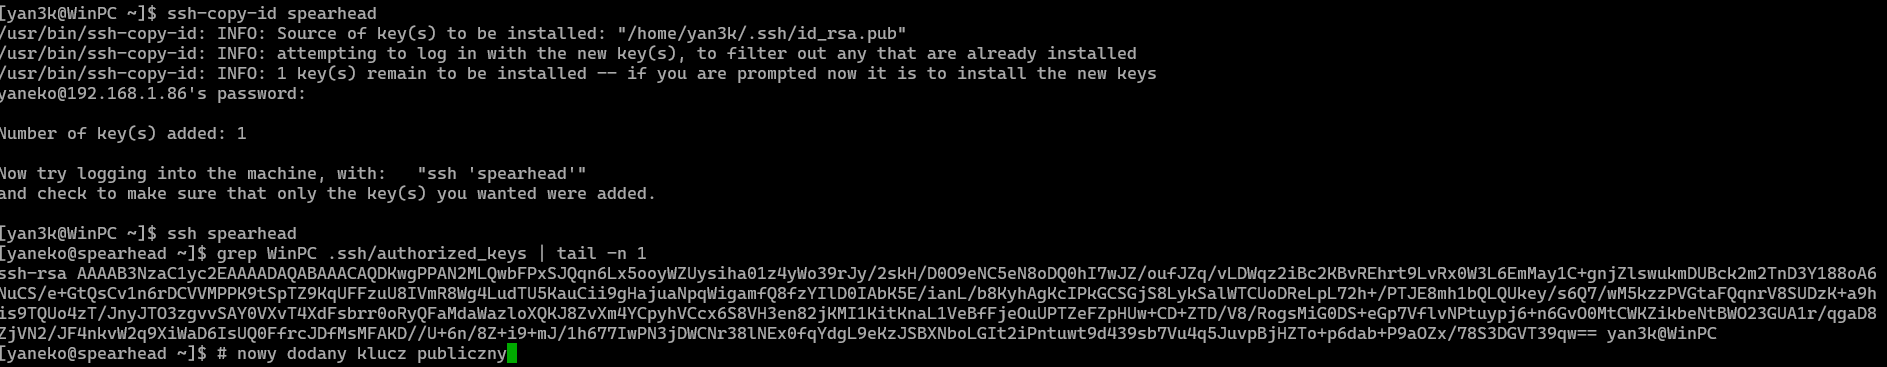
\includegraphics[width=\linewidth]{ssh_copy_id.png}

Powoduje to dodanie zawartości klucza \verb|~/.ssh/id_rsa.pub| (lub innego domyślnego klucza) do \verb|~/.ssh/authorized_keys| na serwerze. Jeśli narzędzie nie jest dostępne, można wykonać ręcznie: najpierw zalogować się hasłem, a potem na serwerze stworzyć katalog \verb|.ssh| i dopisać klucz, np.: 
\begin{verbatim}
mkdir -p ~/.ssh
echo "$(cat ~/.ssh/id_rsa.pub)"
            >> ~/.ssh/authorized_keys
chmod 700 ~/.ssh
chmod 600 ~/.ssh/authorized_keys
\end{verbatim}

\noindent
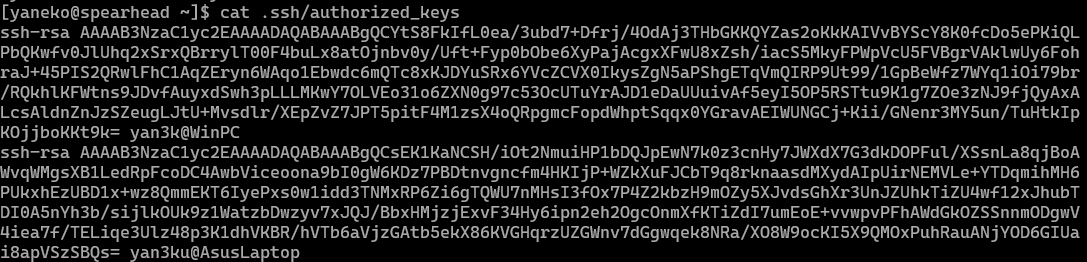
\includegraphics[width=\linewidth]{authorized_keys-linux.png}

Następnie należy zadbać o instalację klucza prywatnego po stronie klienta. W tym celu po wygenerowaniu pary kluczy, plik z kluczem prywatnym (\verb|id_rsa|) powinien zostać skopiowany lub przeniesiony tylko do katalogu domowego użytkownika klienta, w podkatalogu \verb|.ssh|: \verb|mv /path/to/id_rsa ~/.ssh/id_rsa|.

Po dodaniu klucza można przetestować logowanie: \verb|ssh user@serwer| już nie powinno prosić o hasło
(chyba że nadaliśmy passphrase do klucza).

\subsubsection{Klient i serwer SSH Windows (OpenSSH)}
Windows (np. Windows 10) posiada wbudowany serwer OpenSSH (lub Win32-OpenSSH). Konfiguracja kluczy jest analogiczna: klucz publiczny wrzucamy do pliku \verb|authorized_keys|. Dla konta użytkownika domyślnie jest to ścieżka: \verb|C:\Users\<user>\.ssh\authorized_keys|.

\noindent
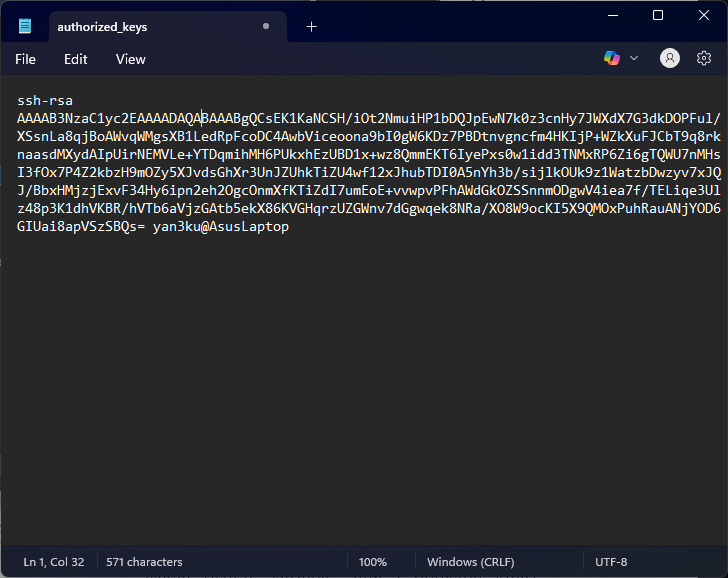
\includegraphics[width=\linewidth]{authorized_keys-win.png}

Dla kont administratora przewidziano specjalny plik w katalogu \verb|C:\ProgramData\ssh\|: \verb|administrators_authorized_keys|. Zawartość tych plików można wprowadzić ręcznie np. przez \verb|scp| lub nawet komendami PowerShell (przykład w dokumentacji Microsoft pokazuje użycie ssh z parametrem, który na zdalnym serwerze tworzy katalog \verb|.ssh| i dopisuje klucz do \verb|authorized_keys|). Ważne jest, aby katalog \verb|.ssh| miał ograniczone prawa (tylko właściciel czy administrator), inaczej OpenSSH może odrzucić klucze.

W tym przypadku plik z kluczem prywatnym powinien trafić analogicznie jak na Linuxie do folderu \verb|.ssh| w foledrze domowym użytkownika: \verb|C:\Users\<user>\.ssh\id_rsa|.


Po umieszczeniu klucza publicznego, logowanie SSH przebiega z użyciem klucza, bez hasła.

\subsubsection{Klient SSH PuTTY}
W przypadku PuTTY klucz prywatny musi być w formacie PuTTY (\verb|.ppk|). Jeżeli mamy klucz w formacie OpenSSH (np. wygenerowany wcześniej ssh-keygenem), wystarczy go załadować w PuTTYgen (Load private key) i zapisać jako \verb|.ppk| (Save private key). Następnie, aby PuTTY użył klucza, w oknie konfiguracji sesji PuTTY przechodzimy do Connection → SSH → Auth i w polu ,,Private key file for authentication'' wybieramy nasz plik \verb|.ppk|.

\noindent
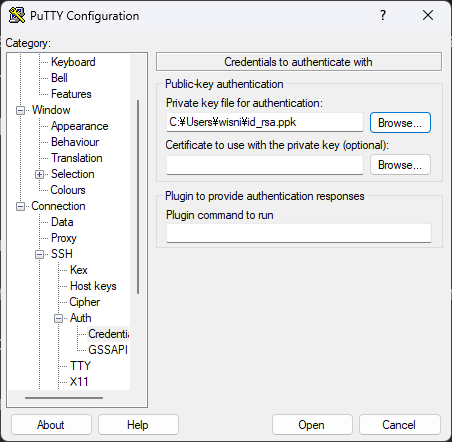
\includegraphics[width=\linewidth]{putty_setting-credentials.png}

W razie potrzeby możemy też użyć Pageanta -- agenta kluczy PuTTY -- i dodać tam klucz. Klucz publiczny PuTTY (tekst z pola ,,Public key for pasting...'' w PuTTYgen) należy skopiować na serwer do \verb|~/.ssh/authorized_keys| tak samo, jak w poprzednich metodach. Po dodaniu klucza do \verb|authorized_keys| należy skonfigurować PuTTY wskazując wygenerowany prywatny plik \verb|.ppk| i przetestować połączenie.

\end{multicols}

\begin{multicols}{2}
[
\section{Zastosowania SSH}
]
\subsection{Zdalny terminal}
Najpopularniejszym zastosowaniem protokołu SSH jest zdalny terminal. SSH umożliwia to, co umożliwia ,,zwykły'' terminal używany lokalnie, lecz przez sieć. Dzięki zdalnemu połączeniu nie trzeba znajdować się fizycznie przy serwerze, żeby sprawdzić np. obecność plików konfiguracyjnych czy status danej usługi.

\noindent
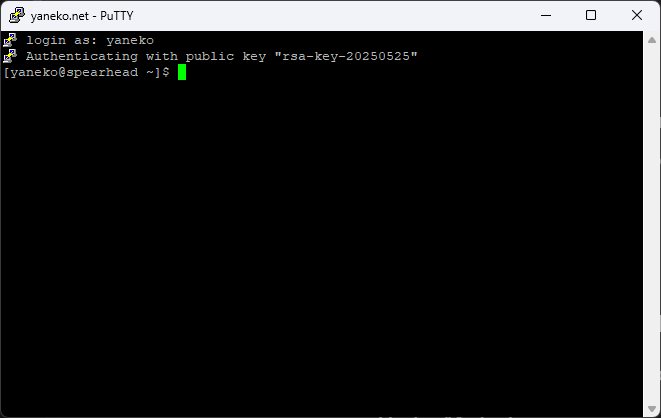
\includegraphics[width=\linewidth]{putty_login-key.png}

\subsection{Przesył plików}
Drugim popularnym zastosowaniem jest transfer plików. Istnieje kilka protokołów tego transferu, opartych na protokole SSH.

\subsubsection{SFTP (Secure FTP)}
SFTP to protokół transferu plików bazujący na SSH. Domyślnie używa tego samego szyfrowanego kanału SSH i tych samych metod uwierzytelniania co SSH. Oznacza to, że jeśli już mamy skonfigurowany klucz dla SSH, wystarczy wpisać w terminalu: \verb|sftp user@host|.

Sesja SFTP rozpocznie się tak samo jak zwykłe połączenie SSH (możemy się spodziewać monitu o passphrase klucza prywatnego, jeśli go ustawiliśmy). Po zalogowaniu otrzymujemy interaktywny prompt \verb|sftp>|, w którym można używać komend typu \verb|ls|, \verb|cd|, \verb|get filename|, \verb|put filename| itp., aby pobierać lub wysyłać pliki\cite{digitalsftp}. 

Ponieważ uwierzytelnienie odbywa się kluczem, SFTP nie będzie już prosić o hasło użytkownika (chyba że klucz miał ustawione hasło).

\subsubsection{SCP (Secure Copy)}
Polecenie scp pozwala kopiować pliki między maszynami z wykorzystaniem SSH. Jeśli autoryzacja kluczem jest skonfigurowana, wystarczy użyć scp tak jak zwykle, np.: 
\begin{verbatim}
  scp lokalny_plik.txt
          user@host:/zdalna/sciezka/
\end{verbatim}

\noindent
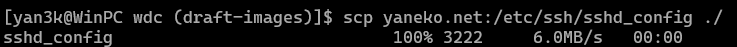
\includegraphics[width=\linewidth]{scp.png}

Ta komenda przeniesie plik na serwer bez potrzeby podawania hasła (chyba że nasz klucz ma passphrase). Po skopiowaniu pliku \verb|scp| wyświetli komunikat o postępie, a przesłany plik znajdziemy w zadanym katalogu na hoście.

\subsubsection{WinSCP}
WinSCP to graficzny klient SFTP/SCP na Windows. Po wybraniu protokołu SFTP wpisujemy dane sesji (nazwa hosta, port, użytkownik). W Advanced (zaawansowanych ustawieniach) przechodzimy do SSH → Authentication i wskazujemy ścieżkę do pliku klucza prywatnego (PuTTY \verb|.ppk|)\cite{superuser}. WinSCP automatycznie użyje tego klucza przy nawiązywaniu połączenia. 

Po udanym zalogowaniu widzimy interfejs drag\&drop dwóch katalogów (lokalnego i zdalnego) – możemy wtedy przeciągać pliki albo używać komend Get i Put jak w SFTP. Dzięki zastosowaniu klucza prywatnego transfer plików przebiega bez pytania o hasło. 

\end{multicols}

\section{Bibliografia}
\renewcommand{\refname}{Artykuły}
\begin{thebibliography}{9}

\bibitem{whatisssh}
    Tatu Ylonen,
    \emph{What is SSH (Secure Shell)?},
    \url{https://www.ssh.com/academy/ssh},
    [dostęp 24.05.2025].
    
\bibitem{learnms}
    Microsoft Learn,
    \emph{Key-based authentication in OpenSSH for Windows},
    \url{https://learn.microsoft.com/en-us/windows-server/administration/openssh/openssh_keymanagement}
    [dostęp 24.05.2025].

\bibitem{openssh10}
    OpenSSH Release Notes,
    \emph{OpenSSH 10.0},
    \url{https://www.openssh.com/txt/release-10.0},
    [dostęp 24.05.2025].

\bibitem{digitalsftp}
    DigitalOcean Community Tutorial,
    \emph{How To Use SFTP to Securely Transfer Files with a Remote Server},
    \url{https://www.digitalocean.com/community/tutorials/how-to-use-sftp-to-securely-transfer-files-with-a-remote-server},
    [dostęp 24.05.2025].

\bibitem{superuser}
    SuperUser forum,
    \emph{How do I get WinSCP to connect to an SSH server with a private key that I specify?},
    \url{https://superuser.com/questions/1644862/how-do-i-get-winscp-to-connect-to-an-ssh-server-with-a-private-key-that-i-specif},
    [dostęp 24.05.2025].
    
\setcounter{firstbib}{\value{enumiv}}
\end{thebibliography}
\renewcommand{\refname}{Dokumentacje techniczne}
\begin{thebibliography}{9}
\setcounter{enumiv}{\value{firstbib}}

\bibitem{rfc4253}
    Chris Lonvick, Tatu Ylonen,
    Styczeń 2006,
    \emph{The Secure Shell (SSH) Transport Layer Protocol},
    \url{https://www.rfc-editor.org/rfc/rfc4253},
    [dostęp 24.05.2025].    

\bibitem{sshconfig}
    OpenBSD manual page server,
    \emph{ssh\_config},
    \url{https://man.openbsd.org/ssh_config},
    [dostęp 24.05.2025].    

\bibitem{sshkeygen}
    OpenBSD manual page server,
    \emph{ssh-keygen},
    \url{https://man.openbsd.org/OpenBSD-current/man1/ssh-keygen},
    [dostęp 24.05.2025].    
    
\end{thebibliography}

\end{document}
